\documentclass{standalone}
\usepackage{tikz}
\usetikzlibrary{arrows, automata}
\begin{document}

	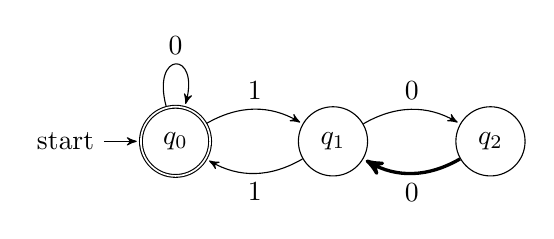
\begin{tikzpicture}[>=stealth',shorten >=1pt,auto,node distance=2cm]
		\node[initial,state,accepting] (0)                {$q_0$};
		\node[state]                   (1) [right of = 0] {$q_1$};
		\node[state]                   (2) [right of = 1] {$q_2$};


		\path[->](0) edge [loop above] node {0} (0);
		\path[->](0) edge [bend left]  node {1} (1);
		\path[->](1) edge [bend left]  node {0} (2);
		\path[->](1) edge [bend left]  node {1} (0);
		\path[->, very thick](2) edge [bend left]  node {0} (1);
	\end{tikzpicture}

\end{document}
